\documentclass[12pt]{article}
\usepackage[utf8]{inputenc}
\usepackage{graphicx}
\usepackage{titling}
\usepackage{datetime}
\usepackage{enumitem}
\usepackage{xcolor}
\usepackage{listings}
\usepackage{multirow}

% Título de la tarea
\title{\vspace{1cm}Proyecto Final de Bases de Datos}
\date{} % Deja la fecha en blanco

% Ajustar márgenes para la portada
\usepackage[left=3cm,right=3cm,top=3cm,bottom=3cm]{geometry}

% Comando para agregar los escudos
\newcommand{\doubleshield}[2]{%
    \begin{minipage}[t]{0.48\textwidth}
        \centering
        \includegraphics[width=0.5\linewidth]{#1}
        \par\vspace{1ex}
        %Escudo #1
    \end{minipage}\hfill%
    \begin{minipage}[t]{0.48\textwidth}
        \centering
        \includegraphics[width=0.5\linewidth]{#2}
        \par\vspace{1ex}
        %Escudo #2
    \end{minipage}%
}

\begin{document}

\lstset{
    language=SQL,                   % Lenguaje de programación
    basicstyle=\ttfamily,              % Fuente y estilo básico
    keywordstyle=\color{red},         % Estilo de las palabras clave
    commentstyle=\color{green},        % Estilo de los comentarios
    numbers=left,                      % Números de línea a la izquierda
    numberstyle=\tiny\color{gray},     % Estilo de los números de línea
    frame=single,                      % Borde alrededor del código
    breaklines=true,                   % Romper líneas largas
    postbreak=\mbox{\textcolor{red}{$\hookrightarrow$}\space}, % Flecha de ruptura de línea
    showstringspaces=false             % No mostrar espacios en cadenas
}


\pagecolor{black}
\color{white}

\begin{titlepage}
    \begin{center}
        \vspace*{2cm}
        
        % Agrega los escudos aquí
        \doubleshield{UNAM.png}{EFC.png}
        
        \vspace{2cm}
        
        \Huge{\thetitle}
        
        \vspace{4cm}
        
        \Large{Tarea presentada por:}
        
        \vspace{0.5cm}
        
        \Large{Edgar Montiel Ledesma 317317794 \\ Carlos Daniel Cortes Jimenez 420004846}
        
        \vfill
        
        Facultad de Ciencias \\
        Universidad Nacional Autónoma de Méixco \\
        Fecha de Entrega: 11 de Diciembre de 2023 % Cambia la fecha de entrega        
    \end{center}
\end{titlepage}
    
    \section*{Base de Datos: Sistema de Administración de Tienda en Línea}

    \subsection*{1. Lista de Requerimientos}
    % Lista de requerimientos aquí
        \begin{itemize}
            \item[1.] Registro de Clientes:
                \begin{itemize}
                    \item La base de datos debe permitir el registro de nuevos clientes, incluyendo su nombre, dirección y número de teléfono.
                \end{itemize}
            \item[2.] Registro de Autos:
                \begin{itemize}
                    \item La base de datos debe permitir el registro de nuevos autos, incluyendo información como modelo, marca, año de fabricación y precio.
                \end{itemize}
            \item[3.] Registro de Empleados:
                \begin{itemize}
                    \item La base de datos debe permitir el registro de empleados, especificando su nombre, dirección, número de teléfono y rol en la agencia (gerente, asesor, promotor, mecánico, electromecánico, etc.).
                \end{itemize}
            \item[4.] Registro de Servicios:
                \begin{itemize}
                    \item La base de datos debe permitir el registro de servicios ofrecidos por la agencia, incluyendo nombre del servicio, descripción y precio.
                \end{itemize}
            \item[5.] Registro de Mantenimientos:
                \begin{itemize}
                    \item La base de datos debe permitir el registro de mantenimientos realizados, especificando el auto involucrado, el cliente, el empleado a cargo, el servicio proporcionado y la fecha del mantenimiento.
                \end{itemize}
            \item[6.] Registro de Trabajos de Hojalatería y Pintura:
                \begin{itemize}
                    \item La base de datos debe permitir el registro de trabajos de hojalatería y pintura, indicando el auto, el cliente, el empleado responsable, el servicio proporcionado y la fecha del trabajo.
                \end{itemize}
            \item[7.] Registro de Seguros para Autos:
                \begin{itemize}
                    \item La base de datos debe permitir el registro de seguros para autos, detallando el auto asegurado, el cliente, el tipo de seguro, la cobertura y el precio del seguro.
                \end{itemize}
            \item[8.] Relaciones entre Entidades:
                \begin{itemize}
                    \item La base de datos debe establecer y mantener relaciones adecuadas entre las entidades, como la asociación de autos con clientes, empleados con mantenimientos y servicios con mantenimientos.
                \end{itemize}
            \item[9.] Consulta de Información:
                \begin{itemize}
                    \item Debe ser posible realizar consultas para obtener información detallada, como el historial de mantenimientos de un auto, los clientes asociados a un empleado.
                \end{itemize}
            \item[10.] Integridad Referencial:
                \begin{itemize}
                    \item La base de datos debe garantizar la integridad referencial, asegurando que las claves foráneas estén correctamente vinculadas a las claves primarias correspondientes.
                \end{itemize}
            \item[11.] Manejo de Precios en Decimal:
                \begin{itemize}
                    \item Los precios deben manejarse con precisión decimal, considerando los campos que almacenan valores monetarios.
                \end{itemize}
            \item[12.] Registro de Fechas:
                \begin{itemize}
                    \item La base de datos debe almacenar fechas de manera precisa para rastrear la temporalidad de eventos como mantenimientos, trabajos de hojalatería y pintura.
                \end{itemize}
        \end{itemize}

    \subsection*{2. Modelo Conceptual (Notación de Peter Chen)}
    \begin{figure}[h]
        \centering
        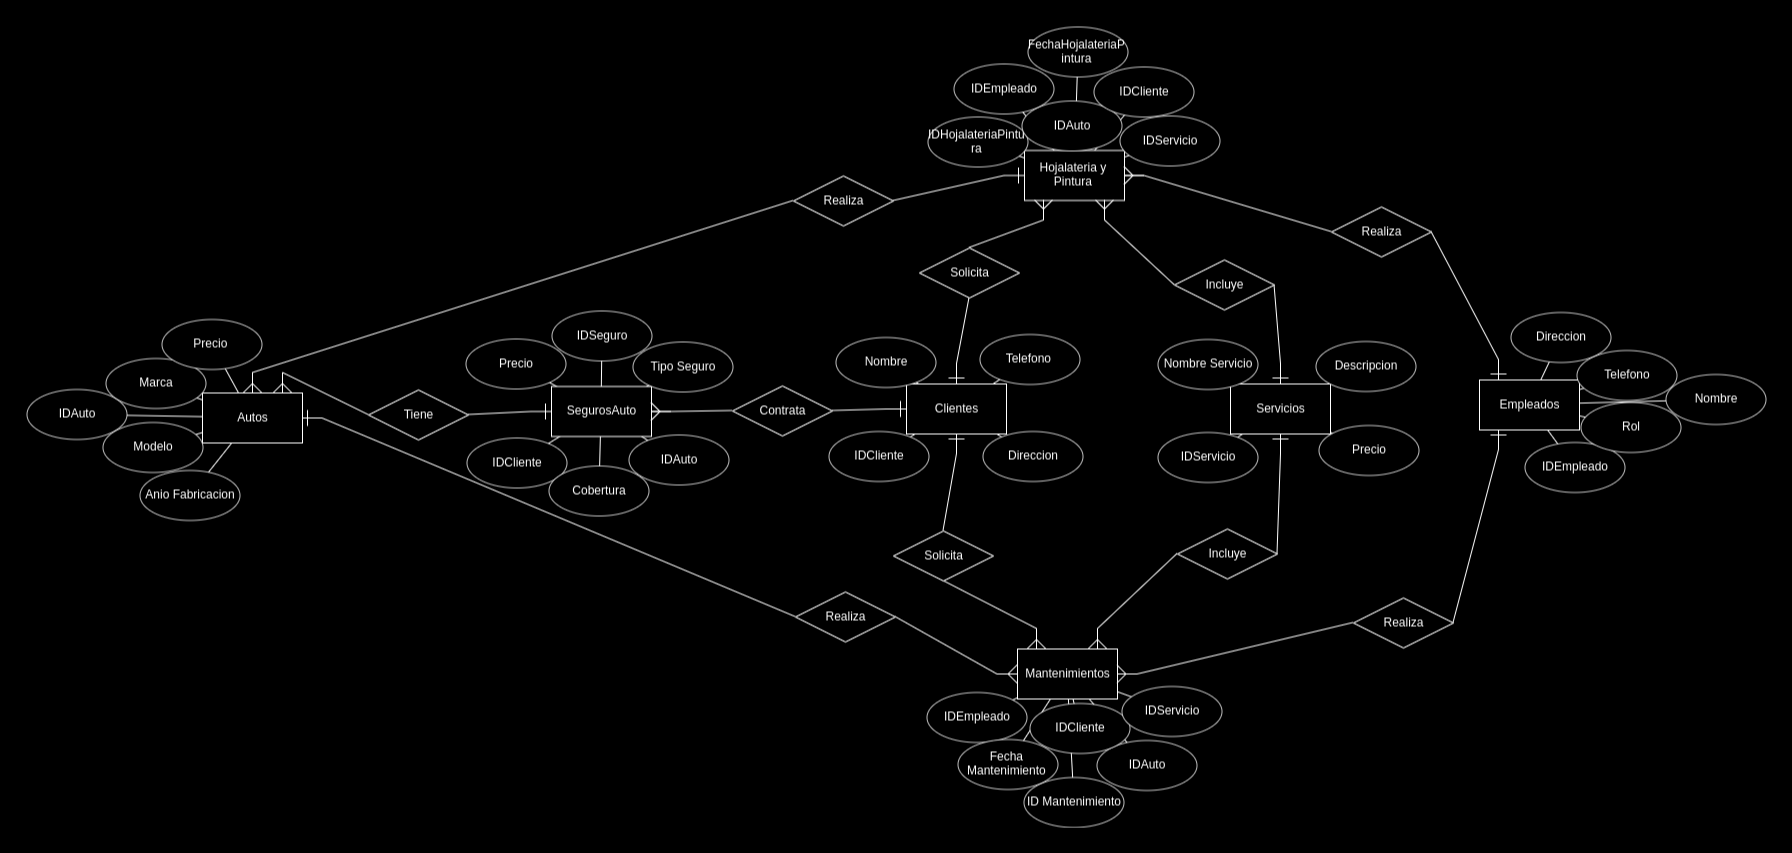
\includegraphics[width=0.9\textwidth]{EAuto.png}
        \caption{Modelo Conceptual}
        \label{fig:modelo-conceptual}
    \end{figure}

    \subsection*{3. Modelo Relacional}
    \begin{figure}[h]
        \centering
        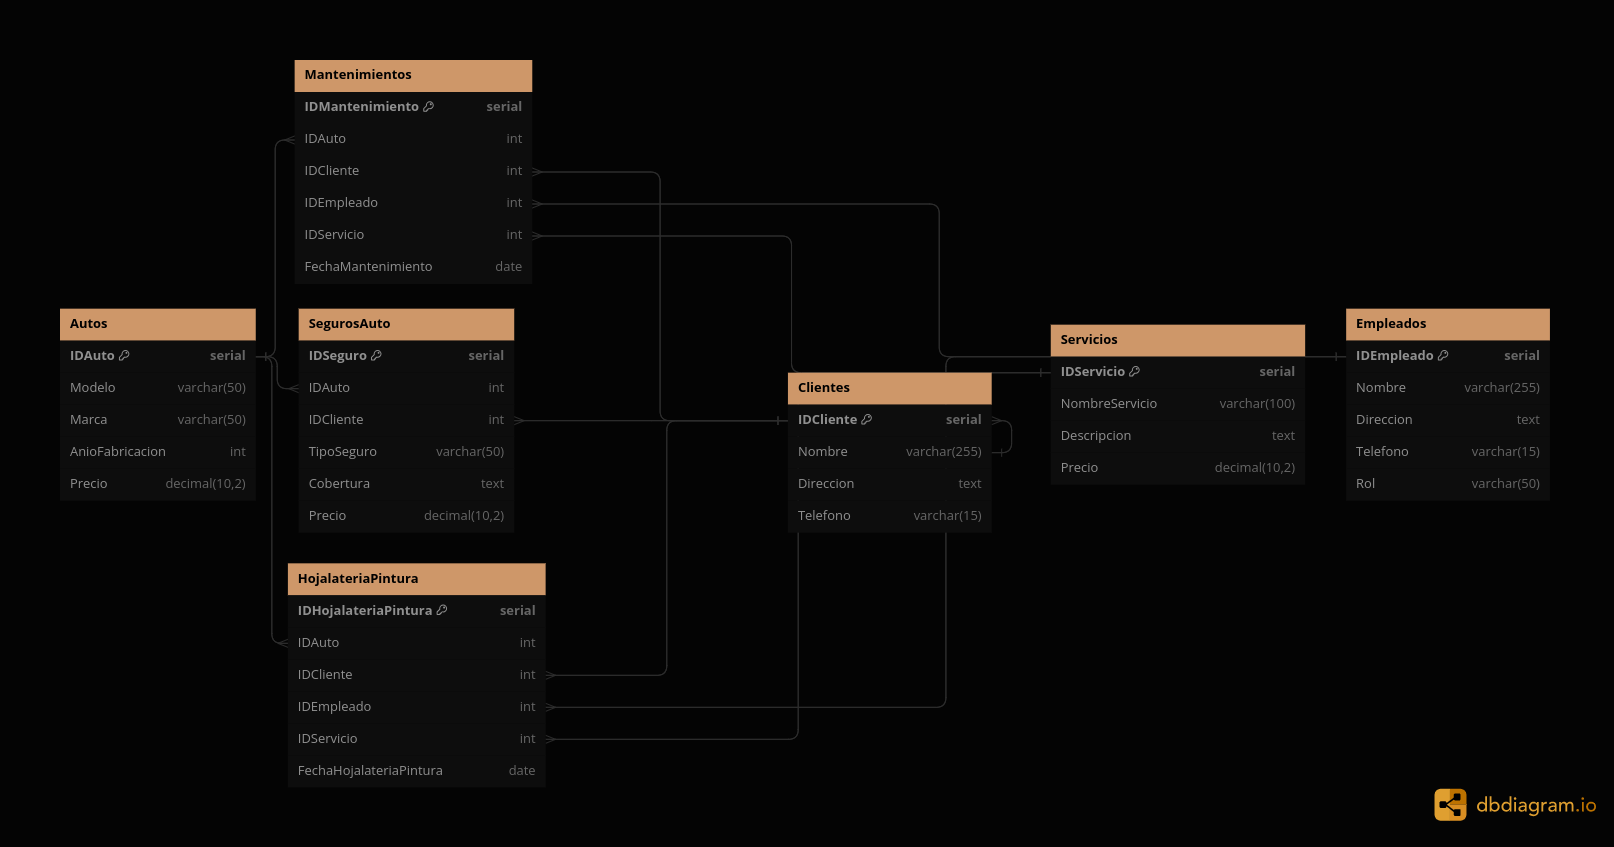
\includegraphics[width=1.0\textwidth]{ERAuto.png}
        \caption{Modelo Conceptual}
        \label{fig:modelo-conceptual}
    \end{figure}

    \subsection*{4. Script Completo para Crear la Base de Datos}
    \begin{lstlisting}[language=SQL]
CREATE TABLE "Clientes" (
  "IDCliente" serial PRIMARY KEY,
  "Nombre" varchar(255),
  "Direccion" text,
  "Telefono" varchar(15)
);

CREATE TABLE "Autos" (
  "IDAuto" serial PRIMARY KEY,
  "Modelo" varchar(50),
  "Marca" varchar(50),
  "AnioFabricacion" int,
  "Precio" decimal(10,2)
);

CREATE TABLE "Empleados" (
  "IDEmpleado" serial PRIMARY KEY,
  "Nombre" varchar(255),
  "Direccion" text,
  "Telefono" varchar(15),
  "Rol" varchar(50)
);

CREATE TABLE "Servicios" (
  "IDServicio" serial PRIMARY KEY,
  "NombreServicio" varchar(100),
  "Descripcion" text,
  "Precio" decimal(10,2)
);

CREATE TABLE "Mantenimientos" (
  "IDMantenimiento" serial PRIMARY KEY,
  "IDAuto" int,
  "IDCliente" int,
  "IDEmpleado" int,
  "IDServicio" int,
  "FechaMantenimiento" date
);

CREATE TABLE "HojalateriaPintura" (
  "IDHojalateriaPintura" serial PRIMARY KEY,
  "IDAuto" int,
  "IDCliente" int,
  "IDEmpleado" int,
  "IDServicio" int,
  "FechaHojalateriaPintura" date
);

CREATE TABLE "SegurosAuto" (
  "IDSeguro" serial PRIMARY KEY,
  "IDAuto" int,
  "IDCliente" int,
  "TipoSeguro" varchar(50),
  "Cobertura" text,
  "Precio" decimal(10,2)
);
    \end{lstlisting}

    \subsection*{5. Script de Inserción de Datos (para 100 registros)}
    Tabla "Clientes" 
    \begin{lstlisting}[language=SQL]
        -- Incluir aqui las instrucciones INSERT para las tablas.
    \end{lstlisting}

    Tabla "Clientes" 
    \begin{lstlisting}[language=SQL]
        -- Incluir aqui las instrucciones INSERT para las tablas.
    \end{lstlisting}

    Tabla "Clientes" 
    \begin{lstlisting}[language=SQL]
        -- Incluir aqui las instrucciones INSERT para las tablas.
    \end{lstlisting}

    Tabla "Clientes" 
    \begin{lstlisting}[language=SQL]
        -- Incluir aqui las instrucciones INSERT para las tablas.
    \end{lstlisting}

    Tabla "Clientes" 
    \begin{lstlisting}[language=SQL]
        -- Incluir aqui las instrucciones INSERT para las tablas.
    \end{lstlisting}

    Tabla "Clientes" 
    \begin{lstlisting}[language=SQL]
        -- Incluir aqui las instrucciones INSERT para las tablas.
    \end{lstlisting}

    Tabla "Clientes" 
    \begin{lstlisting}[language=SQL]
        -- Incluir aqui las instrucciones INSERT para las tablas.
    \end{lstlisting}

    \subsection*{6. Evidencia de Restricciones de Integridad Referencial}
    % Incluir evidencias aquí

    \subsection*{7. Evidencia de Restricciones CHECK}
    % Incluir evidencias aquí
    
    \subsection*{8. Evidencia de Dominios Personalizados}
    % Incluir evidencias aquí
    
    \subsection*{9. Evidencia de Restricciones para Tuplas}
    % Incluir evidencias aquí
    
    \subsection*{10. Consultas Relevantes}
    % Consultas aquí
    
    \subsection*{11. Vistas Relevantes}
    % Vistas aquí
\end{document}

